\documentclass[11pt]{article}
\usepackage[style=apa]{biblatex}
\DeclareLanguageMapping{english}{english-apa} % Resolve labelyearlabelmonthlabelday errors.
\AtEveryBibitem{\clearfield{note}} % Clear note fields.
\usepackage{listings}
\usepackage{enumitem}
\usepackage{lipsum}
\usepackage[symbol]{footmisc}
\usepackage{graphicx}
\usepackage[capposition=top]{floatrow}
\usepackage{listings}
\usepackage{hyperref}
\usepackage{bibentry}
\usepackage[letterpaper, left=1in,top=1in,right=1in,bottom=1in]{geometry}
\usepackage{setspace}
\usepackage{epstopdf}
\usepackage{amssymb}
\usepackage{lineno}
\usepackage{wrapfig}
\usepackage{amsmath}
\usepackage{array}
\usepackage{color,soul}
\usepackage{tabularx}
\usepackage{rotating}
\usepackage{lscape}
\usepackage{subcaption}
\usepackage{longtable}
\usepackage[group-separator={,}, group-minimum-digits=3]{siunitx}
\usepackage{appendix}
\usepackage{pdfpages}
\usepackage{titlesec}
\usepackage{mfirstuc}
\usepackage{multirow}
\usepackage{threeparttable}
\usepackage{color,soul}
\usepackage{todonotes}
\usepackage{mathptmx} % almost times new roman font.
\usepackage{arydshln} % Dashed line.
\usepackage{enumitem} % enumerate line space.


\renewcommand{\baselinestretch}{1.5}
\renewcommand{\thefootnote}{\arabic{footnote}}
\bibliography{../reference/classification.bib}
% \bibliography{../reference/algorithms/ml_algorithms.bib}
\setcounter{tocdepth}{2}
\onehalfspacing

\usepackage{ragged2e}
\setlength{\RaggedRightParindent}{\parindent}

% 

\title{{\textsc{Classifying nonprofits using supervised machine-learning: Benchmark and guide for social scientists solving real-world problems}}}
\author{%
\textsc{Ji Ma and Isha Kanani} \thanks{J.M.: maji@austin.utexas.edu, LBJ School of Public Affairs and RGK Center for Philanthropy and Community Service; I.K.: ishakanani@utexas.edu, School of Information.} \\[1ex] % Your name \thanks{}
\normalsize University of Texas at Austin \\ % Your institution
% \normalsize {Email: maji@austin.utexas.edu} \\ % Your email address
}


\date{\today} % Leave empty to omit a date \today

%----------------------------------------------------------------------------------------

\begin{document}

\RaggedRight

\maketitle

\begin{abstract}

This research classified the nonprofit organizations in the United States using supervised machine-learning algorithms according to text descriptions, built a workflow and benchmark of applying computational linguistics for future sociological studies, and can help researchers to profile a more accurate civil society. We achieved 83\% overall accuracy for classifying the nonprofits into 10 broad categories, and 78\% for classifying them into 25 major groups. Our study suggests that, machine-learning algorithms, Neural Networks in particular, can substantially and reliably improve researchers' productivity as they can approximate or even outperform human coders on many categories. Therefore, human researchers can focusing on the categories on which the algorithms have poor performance. We provided a clear strategy and operationalization method on how machine-learning classifiers can ``complement'' human researchers. A Python software package was developed for scholars. Practical suggestions and future directions are discussed. 

\end{abstract}
\clearpage

% \listoftodos
\tableofcontents
\listoftables
\listoffigures
\clearpage

\section{Introduction}

Although the voluntary and philanthropic organizations have long been existent for numerous centuries, the so-called ``nonprofit sector'' was only coined in the 1970s by scholars, policy makers, and nonprofit practitioners \parencite{HallHistoricalOverviewPhilanthropy2006}. A major reason for assembling the diverse organizations as a conceptual whole is to legitimize the existence of these organizations and the benefits these organizations receive \parencites[54-55]{HallHistoricalOverviewPhilanthropy2006}{BarmanClassificatoryStrugglesNonprofit2013}. From Durkheim's (\citeyear{DurkheimElementaryFormsReligious2012}) perspective, the order and structure of a society can be reflected by a classification system. The National Taxonomy of Exempt Entities (NTEE) developed by the National Center for Charitable Statistics (NCCS), the most widely used classification system, is one of the efforts legitimizing the existence of nonprofit sector \parencite{Hodgkinsonnewresearchplanning1991,HodgkinsonMappingnonprofitsector1990}. As \textcite[105]{BarmanClassificatoryStrugglesNonprofit2013} cite \textcite[601]{ClarkeSimpleTechnologyComplex1996}: ``The ways in which different entities (people, animals, plants, diseases, etc.) are organized into classificatory groups reveal something of the social, cultural, symbolic, and political contexts within which classifications occur.''

The development of NTEE classifications can date back to the 1980s \parencite[8-9, 11]{HodgkinsonMappingnonprofitsector1990}. In 1982, NCCS assembled a team of experts working on creating a taxonomy for nonprofit organizations. The first draft of the taxonomy, entitled ``National Taxonomy of Exempt Entities'' (NTEE), came out in 1986 and published in 1987. In the early 1990s, NCCS had classified nearly one million nonprofits using NTEE. In 1995, the Internal Revenue Service (IRS) adopted the NTEE coding system, took over the tasks of assigning and maintaining the classifications, and started to release the Business Master File with NTEE codes \parencite{USInternalRevenueServiceExemptOrganizationsBusiness2014,USInternalRevenueServiceIRSStaticFiles2013}.

Two agencies took the task of assigning NTEE codes: NCCS and IRS. Before 1995, NCCS coded nonprofits according to the program descriptions in Part III and VIII of Form 990, supplemented with information from Form 1023 (``Application for Recognition of Exemption'') and additional research \parencite[16]{NationalCenterforCharitableStatisticsGuideUsingNCCS2006}. After 1995, IRS began to issue ``new exempt organizations an NTEE code as part of the determination process,'' and ``the determination specialist assigns an NTEE code to each organization exempt under I.R.C. \S 501(a) as part of the process of closing a case when the organization is recognized as tax-exempt'' \parencite[1]{USInternalRevenueServiceIRSStaticFiles2013}.

The NTEE classification system supported many applied and academic researches on nonprofit organizations which have critical economic and political roles in society. For example, NTEE provides a framework on which the social and economic activities of civil society can be mapped and compared with other sectors in a society \parencite[e.g.,][]{RoegerNonprofitSectorIts2015}. Scholars use NTEE codes to sample the nonprofits of their interests \parencite[e.g.,][]{OktenDeterminantsdonationsprivate2000,SharkeyCommunityCrimeDecline2017,McVeighStructuralInfluencesActivism2006,VasiNoFrackingWay2015} or as independent variables \parencite{SloanEffectsNonprofitAccountability2009}. NTEE can also serve as an analytical tool for measuring the organizational capacity in different service domains and inform practitioners and policymakers' decision-making \parencite{Hodgkinsonnewresearchplanning1991}. The invention of NTEE also provides a fundamental necessity for comparative international research, facilitating the study of ``global civil society'' \parencite{VakilConfrontingclassificationproblem1997,Salamonsearchnonprofitsector1992,Salamoninternationalclassificationnonprofit1996,HodgkinsonMappingnonprofitsector1990}.

The NTEE classification system, although one of the best we have so far, still has several drawbacks. First, because it only assign one major category code to an organization, it cannot accurately describe a nonprofit's programs which are usually diverse and across several service domains \parencite[303]{GronbjergUsingNTEEclassify1994}. Although a program classification system was developed later \parencite{LampkinIntroducingNonprofitProgram2001}, it is not widely used probably because it is impractical to assign codes to massive amount of programs.

Second, the assignment of NTEE codes is not complete because it is ``based on an assessment of program descriptions contained in Parts 3 and 8 of the Form 990'' and ``program descriptions were only available for some organizations'' \parencite[16]{NationalCenterforCharitableStatisticsGuideUsingNCCS2006}. A recent study found the number of organizations in Washington State with a specific NTEE code could be significantly increased if the mission statements were used for coding \parencite{FyallNTEECodesOpportunities2018}.

Third, NTEE codes are static but nonprofit organizations' activities may change over time. Recoding existent NTEE assignments is extremely onerous, and this may be one of the reason that IRS does not have a procedure by which the nonprofits can request the change of their NTEE codes \parencite{USInternalRevenueServiceIRSStaticFiles2013}.

Fourth, a vast amount of grassroots organizations are not classified and missing in existing datasets because organizations ``that normally has annual gross receipts of \$50,000 or less'' are not required to report to IRS \parencite{USInternalRevenueServiceAnnualExemptOrganization2019}. As \textcite{SmithRestNonprofitSector1997} estimates, the IRS listings ignore about 90\% nonprofits of which most are grassroots associations. The organizational activities at grassroots level are particularly important for sociological and political studies, and most studies fail to consider these grassroots organizations because of dataset limitation \parencite[e.g.,][]{McVeighStructuralInfluencesActivism2006,VasiNoFrackingWay2015,SharkeyCommunityCrimeDecline2017}.

The tremendous human labor needed for classification is a prominent challenge, and such challenge is also an evident barrier for improving any classification system. Numerous social scientists experimented with applying computational methods in classifying objects for solving real-world problems \parencite[e.g.,][]{BacakPrincipledMachineLearning2018,NelsonFutureCodingComparison2018,FyallNTEECodesOpportunities2018,GrimmerTextDataPromise2013}. We respond to the challenge by applying the advances in computational linguistics and made the following contributions to the growing literature: 1) we established a standardized workflow and benchmarks which future studies of nonprofit or classification in other social science disciplines can build on and compare to; 2) we achieved {83\%} overall accuracy for classifying the nonprofits into 10 broad categories, and {78\%} for classifying them into 25 major groups; 3) we developed a Python software package for scholars to classify text descriptions using NTEE codes; 4) we released all source codes, data, and work history for replication purposes and future studies, this is particularly important since there are many caveats in tuning algorithms which cannot be detailed in this paper.\footnote{Follow this link for the complete working directory with detail instructions: https://github.com/***}


\section{Method}

Classifying texts is a typical task of automatic content analysis and usually employs three types of methods: dictionary, supervised, and unsupervised methods \parencite[268-269]{GrimmerTextDataPromise2013}. The dictionary methods use a predefined dictionary of words to classifying the texts. Although accurate, this approach is not capable to deal with the variations and contexts of language. The supervised method is an improved solution which uses computer algorithms to ``learn'' the linguistic patters in a dataset classified by human coders. Unlike the dictionary and supervised methods which require predefined categories of interest, unsupervised methods can discover linguistic patters in texts without inputting any knowledge of classification. However, unsupervised method's validity can be problematic because the returned classifications may not be theoretically meaningful. To take the advantage of existing human-coded NTEE classifications and the experience of existing studies \parencite{NelsonFutureCodingComparison2018,FyallNTEECodesOpportunities2018}, this study employs a supervised approach as Figure \ref{fig:workflow} illustrates.

\begin{figure}
	\centering
	\caption{\textsc{Research workflow}} \label{fig:workflow}
	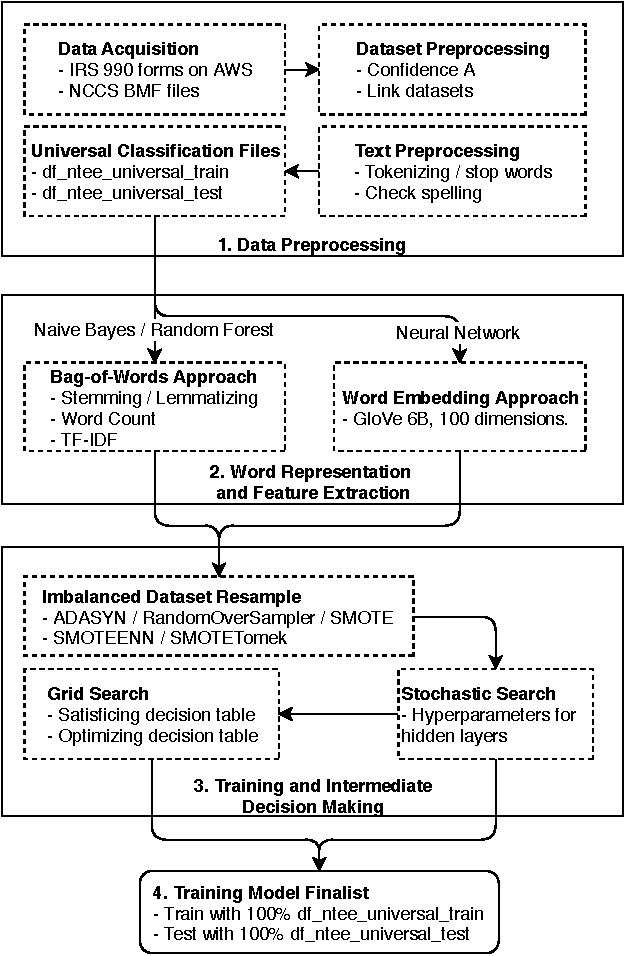
\includegraphics[width=0.7\textwidth]{tbl_fig/ntee_classification.pdf}
\end{figure}

Figure \ref{fig:workflow} presents this paper's complete workflow. We implement four stages of analysis: 1) \textit{preprocessing stage} includes data acquisition and the preprocessing of datasets and texts; 2) \textit{feature extraction} includes bag-of-words (used by Naive Bayes and Random Forest algorithms) and word embedding (used by neural network algorithms); 3) at \textit{training and intermediate decision making} phase, we use stochastic and grid search to train, search, and optimize the machine learning algorithms; 4) we \textit{train the model finalist} with the complete dataset and prepare the trained model for public use. The following part introduces the four phases in detail.

\subsection{Data preprocessing}

\begin{table}[]
    \centering
    \begin{tabularx}{0.8\textwidth}{r|X|X}
    	 \hline
         & Mission Statement & Program Description \\
         \hline
         990 & Part I, Line 1; Part III, Line 1 & Part III, Line 4; Part VIII, Line 2a-e, Line 11a-c; Schedule O \\
         \hdashline
         990-EZ & Part III & Part III, Line 28-30; Schedule O \\
         \hdashline
         990-PF & -- & Part IX-A; Part XVI-B \\
         \hline
    \end{tabularx}
    \caption{\textsc{Locations of text fields in different forms}} \label{tab:text_loc}
\end{table}

\textit{Data acquisition and dataset preprocessing.} We collected text records from form 990, 990-EZ, and 990-PF, and supplemented these records with program descriptions from Schedule O. Form 990 (Return of Organization Exempt From Income Tax) is submitted by most of the nonprofit organizations. For smaller organizations with ``gross receipts of less than \$200,000 and total assets of less than \$500,000 at the end of their tax year'' \parencite[1]{USInternalRevenueService2017InstructionsForm2018}, they can file Form 990-EZ (Short Form Return of Organization Exempt From Income Tax), a shorter version of Form 990. Private foundations use Form 990-PF (Return of Private Foundation). The texts describes organizational activities in two forms: overall mission statement and specific program description. Table \ref{tab:text_loc} summarizes these text fields' specific locations in different forms.

Classification records (i.e., NTEE codes) are collected from the 2014-2016 Business Master Files on NCCS website.\footnote{https://nccs-data.urban.org} This study deals with two types of NTEE classifications: 10 broad category and 26 major groups. Table \ref{tab:classification} shows the relationship between broad categories and major groups. A detail list of the 26 major groups can be found in \textcite{USInternalRevenueServiceExemptOrganizationsBusiness2014}. The accuracy of classification is indicated by a letter of A, B, or C, and ``confidence level of A ... indicates that there is at least a 90 percent probability that the major group classification is correct'' \parencite[16]{NationalCenterforCharitableStatisticsGuideUsingNCCS2006}. The intercoder reliability of records at confidence A level should approximate 100\% \parencite[147]{StengelGettingItRight1998} -- this measure is particularly important because the NTEE codes were assigned by human coders from different organizations (i.e., IRS and NCCS) over different periods of time.

From 2014 to 2016, 56.12\% records are classified at A level, 37.32\% at B level, and 6.56\% at C level. For training purposes, we only use records at confidence level A and drop all X/Z category (i.e., unknown or unclassified). About 1.76\% organizations changed their NTEE codes between 2014 and 2016. We dropped the records of these organizations since these records are less credible.

\begin{table}[]
    \centering
    \begin{tabularx}{0.9\textwidth}{r|X|X}
    	 \hline
         Broad Category Code & Explanation & Major Group Code \\
         \hline
		I & Arts, Culture, and Humanities & A \\
		II & Education & B \\
		III & Environment and Animals & C, D \\
		IV & Health & E, F, G, H \\
		V & Human Services & I, J, K, L, M, N, O, P \\
		VI & International, Foreign Affairs & Q \\
		VII & Public, Societal Benefit & R, S, T, U, V, W \\
		VIII & Religion Related & X \\
		IX & Mutual/Membership Benefit & Y \\
		X & Unknown, Unclassified & Z \\
         \hline
    \end{tabularx}
    \caption{\textsc{NTEE-CC classification system}} \label{tab:classification}
\end{table}


\textit{Text Preprocessing.} Texts in sentences need to be ``tokenized'' into words before analysis, which is called ``tokenization'' in natural language processing. We also removed stop words (e.g., ``the'', ``a'' and punctuation marks) and checked spelling errors using algorithms based on ``minimum edit distance'' (ie., the minimum number of editing operations needed to change one word into another; \textcite[26]{JurafskySpeechLanguageProcessing2017}).

\textit{Universal Classification Files (UCFs).} The final step at data preprocessing stage is to divide data records into training and testing datasets (i.e., files in \texttt{/dataset/df\_ntee\_universal/}) that are mutually exclusive and can be used for benchmarking future models. The \textit{Universal Classification File Training} (UCF-Training) (\texttt{df\_ntee\_universal\_train.pkl.gz}) is used for developing models and consists of 80\% total records. The \textit{Universal Classification File Testing} (UCF-Testing) (\texttt{df\_ntee\_universal\_test.pkl.gz}) is used for testing trained models' performance and consists of 20\% total records. Table \ref{tab:universal_file} presents the two datasets' composition by major groups. The UCFs approximate the composition of organizations reported to the IRS except group A (``arts, culture, and humanities'') and T (``philanthropy, voluntarism, and grantmaking foundations''). The consequence is that, comparing to human coders, the trained models are less likely to categorize organizations as T but more likely to categorize organizations as A.

\begin{table}[t]
    \centering
    \begin{threeparttable}
    \caption{\textsc{Composition of Universal Classification Files}} \label{tab:universal_file}
    \begin{tabularx}{\textwidth}{c|r|r|r|r|r|r}
    	 \hline
         Major Group & Training (\#) & Training (\%) & Testing (\#) & Testing (\%) & Reported (\#) & Reported (\%) \\
         \hline
			A & \num{17010} & \num{11.02}\% & \num{4291} & \num{11.11}\% & \num{35813} & \num{6.77}\% \\
			\hdashline
			B & \num{25827} & \num{16.72}\% & \num{6419} & \num{16.63}\% & \num{67879} & \num{12.83}\% \\
			\hdashline
			C & \num{3323} & \num{2.15}\% & \num{827} & \num{2.14}\% & \num{9054} & \num{1.71}\% \\
			D & \num{4239} & \num{2.75}\% & \num{1034} & \num{2.68}\% & \num{8740} & \num{1.65}\% \\
			\hdashline
			E & \num{9015} & \num{5.84}\% & \num{2307} & \num{5.98}\% & \num{25643} & \num{4.85}\% \\
			F & \num{2301} & \num{1.49}\% & \num{543} & \num{1.41}\% & \num{8481} & \num{1.60}\% \\
			G & \num{5053} & \num{3.27}\% & \num{1353} & \num{3.50}\% & \num{10697} & \num{2.02}\% \\
			H & \num{467} & \num{0.30}\% & \num{126} & \num{0.33}\% & \num{2203} & \num{0.42}\% \\
			\hdashline
			I & \num{2947} & \num{1.91}\% & \num{740} & \num{1.92}\% & \num{8687} & \num{1.64}\% \\
			J & \num{4772} & \num{3.09}\% & \num{1132} & \num{2.93}\% & \num{15841} & \num{2.99}\% \\
			K & \num{2009} & \num{1.30}\% & \num{522} & \num{1.35}\% & \num{7444} & \num{1.41}\% \\
			L & \num{5942} & \num{3.85}\% & \num{1537} & \num{3.98}\% & \num{20428} & \num{3.86}\% \\
			M & \num{4693} & \num{3.04}\% & \num{1140} & \num{2.95}\% & \num{10857} & \num{2.05}\% \\
			N & \num{15460} & \num{10.01}\% & \num{3925} & \num{10.17}\% & \num{43987} & \num{8.31}\% \\
			O & \num{1731} & \num{1.12}\% & \num{409} & \num{1.06}\% & \num{7878} & \num{1.49}\% \\
			P & \num{9180} & \num{5.94}\% & \num{2318} & \num{6.00}\% & \num{40880} & \num{7.73}\% \\
			\hdashline
			Q & \num{1987} & \num{1.29}\% & \num{436} & \num{1.13}\% & \num{7288} & \num{1.38}\% \\
			\hdashline
			R & \num{1064} & \num{0.69}\% & \num{257} & \num{0.67}\% & \num{2830} & \num{0.53}\% \\
			S & \num{14459} & \num{9.36}\% & \num{3603} & \num{9.33}\% & \num{48387} & \num{9.14}\% \\
			T & \num{2032} & \num{1.32}\% & \num{541} & \num{1.40}\% & \num{84338} & \num{15.94}\% \\
			U & \num{1000} & \num{0.65}\% & \num{225} & \num{0.58}\% & \num{3039} & \num{0.57}\% \\
			V & \num{350} & \num{0.23}\% & \num{85} & \num{0.22}\% & \num{940} & \num{0.18}\% \\
			W & \num{8357} & \num{5.41}\% & \num{2038} & \num{5.28}\% & \num{20862} & \num{3.94}\% \\
			\hdashline
			X & \num{4566} & \num{2.96}\% & \num{1098} & \num{2.84}\% & \num{20699} & \num{3.91}\% \\
			\hdashline
			Y & \num{6640} & \num{4.30}\% & \num{1701} & \num{4.41}\% & \num{15712} & \num{2.97}\% \\
			\hdashline
			Z & -- & -- & -- & -- & \num{547} & \num{0.10}\% \\
			\hline
			Total & \num{154424} & \num{100.00}\% & \num{38607} & \num{100.00}\% & \num{529154} & \num{100.00}\% \\
         \hline
    \end{tabularx}
    \begin{tablenotes}
    \item\footnotesize \textit{Note}: Numbers and percentages reported to the Internal Revenue Service (i.e., last two columns) are from \textcite{McKeeverNonprofitAlmanacEssential2016}. Dashed lines separate the ten broad categories.
    \end{tablenotes}
    \end{threeparttable}
\end{table}

\subsection{Word representation and feature extraction}

The machine learning algorithms can only work on numeric vectors that are transformed from the tokenized sentences. A variety of transformation methods can ``represent'' words as vectors, and good methods should be able to easy the process of extracting ``features'' from texts. In general, there are two approaches to word representation: bag-of-words and word embedding.

\subsubsection{Bag-of-words approach}

Bag-of-words approach considers words in texts as mutually independent, as a result, disregards the order of words in text. For example, ``we are health service organization'' and ``health organization service are we'' are the same bag-of-words. This approach serves as the basis for developing many simple language models because it can efficiently represent the possibility of word's occurrence in texts \parencite{BengfortAppliedTextAnalysis2018}. We adopt two methods in this study to represent the texts: count vector and Term Frequency-Inverse Document Frequency.

\textit{Count vector} counts the number of occurrences of all the words in a given text. Given a set of statements, the algorithm first builds an index of all unique words from the collection which is called vocabulary index. The algorithm then represent the texts using words' frequencies and vocabulary index. Table \ref{tab:count_vector} presents a simple example of count vectors, in which ``we focus on education'' is represented as vector $[1, 1, 1, 0, 0, 0, 0]$

\begin{table}
\caption{\textsc{Example of Count Vectors}} \label{tab:count_vector}
\begin{tabular}{m{3.9cm}|m{0.9cm}|m{1cm}|m{0.9cm}|m{1.5cm}|m{1cm}|m{1cm}|m{0.8cm}}
    \hline
    statements X vocabulary & we & focus & on & education & health & care & about \\
    \hline
    we focus on education & 1 & 1 & 1 & 0 & 0 & 0 & 0 \\ 
    \hdashline
    health care care  & 0 & 0 & 0 & 0 & 1 & 2 & 0 \\ 
    \hdashline
    we care about & 1 & 0 & 0 & 0 & 0 & 1 & 1 \\ 
    \hline
\end{tabular}
\end{table}

\textit{Term Frequency-Inverse Document Frequency} (TF-IDF) normalizes raw word frequencies using the number of documents in which the word appears. As Eq. \ref{eq:tfidf} presents, $tf_{ij}$ is the frequency of word $i$ in mission statement $j$, weighted by the inverse document frequency (i.e., $idf_i$; Eq. \ref{eq:idf}), where $N^{total}$ is the number of total mission statements and $N^{i}$ is the number of mission statements that word $i$ appears. The underlying assumption of TF-IDF is that the words appear in all statements are not as important as those occur in a limited number of statements \parencite[278]{JurafskySpeechLanguageProcessing2017}.

\begin{equation} \label{eq:tfidf}
 w_{ij} = tf_{ij} \cdot idf_i 
\end{equation}
\begin{equation} \label{eq:idf}
idf_i = log(\frac{N^{total}}{N^{i}})
\end{equation}

We need to ``normalize'' the texts to reduce the vocabulary size before transforming using either count vector or TF-IDF, because the same word can have numerous spelling variations. For example, ``environments,'' ``environmental,'' and ``environment'' represent the same root word (i.e., \textit{stem}) ``environ.'' Otherwise, the ML models will suffer from ``the curse of dimensionality'': as the feature increases, the data becomes more discrete and less informative to decision making \parencite[94]{BellmanAdaptiveControlProcesses2015}. 

The process of finding stems is called ``morphological parsing'' which includes two primary methods: \textit{stemming} and \textit{lemmatizing} \parencite[25]{JurafskySpeechLanguageProcessing2017}. Stemming slices longer strings to smaller ones according to a series of predefined rules. For example, ``ational'' is transformed to ``ate'' in all words ending with the former string. Therefore, stemming tend to have errors of both over- and under-parsing. Lemmatizing is a more advanced method which reduces a word to its stem by analyzing its meaning.

\subsubsection{Word embedding approach}

Disregarding the contexts in which the words appear is an evident drawback of bag-of-words approach. The word embedding approach is an new advancement \parencite{MikolovEfficientEstimationWord2013} and was suggested by \textcite{NelsonFutureCodingComparison2018} as a future direction in sociological studies. It represents words in a multi-dimensional space (i.e., each word has a vector value), in which words that often appear together in texts have closer distance with each other \parencites[][290]{JurafskySpeechLanguageProcessing2017}[][65]{BengfortAppliedTextAnalysis2018}. We can either train our own word vectors which require a large corpus and is time-consuming, or use pre-trained word vectors. In this study, we use the 100-dimension word vectors pre-trained from a corpus of 6 billion word tokens \parencite{PenningtonGloveGlobalVectors2014}.

\subsection{Training and intermediate decision making}

\subsubsection{Imbalanced dataset resampling}

Training using imbalanced dataset like UCF-Training can bias our estimation because machine learning algorithms cannot extract enough information from minority classes (e.g., group H and V). Therefore, resampling the imbalanced dataset to build a more balanced one is crucial for predicting minority classes. We experimented with four strategies of over-sampling (i.e., ADASYN, RandomOverSampler, and SMOTE) and two strategies of over-sampling followed by under-sampling to reduce the noise (i.e., SMOTEENN and SMOTETomek; \cite{LemaitreImbalancedlearnPythonToolbox2017}). The influence of resampling is substantial: the $F_1$ score of predicting minority class major group \textit{Q} were improved from 15\% to over 30\% in our pilot experiments.\footnote{Although major group \textit{Q} and broad category \textit{VI} represent the same group of organizations, for computer algorithms, the classification contexts are different, therefore, performance on this category varies.}

\subsubsection{Classifiers for training}

\textit{Na\"ive Bayes (NB) classifier} is built on Baye\'s theorem. It is one of the simplest classifiers to learn and implement among all machine learning algorithms and built on simple conditional probability principles. The classifier assumes all features extracted from the texts are conditionally independent, which is wrong in most cases. But the classifier is efficient and has proven to be useful for a variety of tasks even on a small dataset \parencites[][76]{JurafskySpeechLanguageProcessing2017}[][277]{GrimmerTextDataPromise2013}. We tested two types of NB classifiers: multinomial and Complement NB classifiers \parencite{RennieTacklingPoorAssumptions2003}.

\textit{Random Forest classifier} is implemented by developing multiple prediction models. Each model in this algorithm is trained by different data, and then all of these models are asked to predict for the same record. A prediction class that is elected by most of these small algorithms is given as the prediction result by the random forest algorithm. It uses the word ``forest'' because each small algorithm trained is a decision tree \parencites[83]{QuinlanInductiondecisiontrees1986}. A decision tree represents a set of questions that usually have Yes/No answers. The process starts from the top of the tree with one question, and based on the answer, we further run down on either one side of the tree, and answer another question and repeat till we reach the end of the tree. Each decision tree is trained on a different training set \parencites[124]{BreimanBaggingpredictors1996}. 

Take our study for example, if we provide 5,000 statements with their NTEE codes to a random forest with five trees, each tree will randomly select a thousand records to train. Each tree includes new words at different levels of the tree. For example, the tree starts with word ``emergency,'' it will have two branches for ``yes'' or ``no,'' leading to another word and so on, till the bottom of the tree where the NTEE code is. Since each tree is trained on a different set, when a record is given for prediction, each tree predicts the class independent of other tree. In total of five class predictions will be collected in this case, and the class which has the highest occurrence in the prediction results is given as the final predicted class by the random forest algorithm. 

Since each decision tree in a Random Forest classifier is provided with a unique set of records for the training purpose, it strengthens the performance of the overall forest. The classifier however is difficult to visually interpret. It takes a little effort to visualize how decision trees work and understand the algorithm, unlike the Na\"ive Bayes approach.

\textit{Neural Network (NN) classification} is built on the concepts of a neuron structure of the human mind. Each neuron in the network is connected to a few other neurons of the network by a numerical value called ``weight.'' The neurons process records each one in turn, and learn by looking at their classification (i.e., NTEE code in this case) with the known previous NTEE codes of records. With every new record the neurons learn, they update the connection value ``weight'' to update the model \parencites[163]{CollobertUnifiedArchitectureNatural2008}. After the network is done processing each record of the training set, it has final weights for each connection between two neurons. When a testing set is provided, the neurons use the final weights to predict the NTEE code. Depending on the architecture of the neurons, we can design a variety of NNs (e.g., the basic fully connected, Recurrent, and Long Short-Term Memory). This study uses Convolutional NN (CNN) following other scholars' recommendation \parencite{ZhangSensitivityAnalysisPractitioners2015}.

\subsubsection{Measuring algorithm performance}

An algorithm's performance can be measured by many metrics, but social scientists particularly concern two questions while solving real-word problems: 1) how many predicted observations are correct (i.e., \textit{precision} calculated by Eq. \ref{precision})? 2) how many observations are correctly predicted (i.e., \textit{recall} calculated by Eq. \ref{recall}). Answering the two questions is critical for social scientists to apply ML research methods, and we will analyze the methodological implications and recommended practices in discussion section.

In Eq. \ref{precision}, $k$ is one of the NTEE codes, $\#Org^{corr}_{k}$ is the number of organizations correctly classified as $k$, and ${\#Org^{pred}_{k}}$ is the number of organizations predicted as $k$. $\#Org^{corr}_{k}$ will always be smaller than or equal to ${\#Org^{pred}_{k}}$ because ML algorithms can hardly predict every observation right. For example, $Precision_{B}=0.75$ indicates that 75\% of all the organizations classified as ``education'' are correct.

\begin{equation} \label{precision}
    Precision_{k}=\frac{Org^{corr}_{k}}{Org^{pred}_{k}}
\end{equation}

Assuming robust human-coders' coding of nonprofits as true value, in Eq. \ref{recall}, $Org^{true}_{k}$ is the number of organizations that belong to $k$ category. For example, $Recall_{B}=0.80$ denotes that 80\% of the organizations classified as ``education'' by robust human-coding are correctly identified by the algorithm.

\begin{equation} \label{recall}
    Recall_{k}=\frac{Org^{corr}_{k}}{Org^{true}_{k}}
\end{equation}

$F_1$ score (Eq. \ref{eq:f1}), the harmonic mean of precision and recall, was introduced to balance the two measures.

\begin{equation} \label{eq:f1}
    F_{1k}=\frac{2 \cdot Precision_{k} \cdot Recall_{k}}{Precision_{k} + Recall_{k}}
\end{equation}


\subsubsection{Intermediate decision making}

The goal of this study is to find the best ML algorithm with appropriate parameters. We can either try some of the configurations randomly (i.e., \textit{stochastic search}), or iterate all possible configurations (i.e., \textit{grid search}). For NB and RF algorithms, we used the latter approach. For NN algorithms, we first used stochastic search to narrow down the configurations of hidden layers, and then conducted a grid search for the input and output layers' parameters using CNN. The grid search for all possible parameters (over 2 million combinations) is impossible even by using one of the most advanced super computing clusters in the world.

We conduced two rounds of grid search. The first found is for \textit{satisficing decision making} in which we only considered the configurations that can perform at the top 5 percent (240 parameter combinations for NB and RF, 7,200 for NN, detail history files are in folder \texttt{output}). Then we ran the second found grid search for \textit{optimizing decision making} in which we increased the values of some parameters to allow the algorithms to reach their performance ceilings. We then choose the best algorithm and parameters for final training.


\section{Results}


\subsection{Selecting the best classifier}

For multi-class classification task (i.e., more than two classes to predict), it is difficult to measure the overall performance because for each category the performance differs. Table \ref{tab:perf_compare} presents the performance of CNN classifiers with and without resampling. Because the dataset is imbalanced, the classifier has a poor performance on category \textit{VI International, Foreign Affairs} without resampling. Training the classifier with resampled dataset substantially improves the $F_1$ score from 14\% to 29\%, but slightly sacrifices the performance on other categories. So which one should we choose?

We choose the classifier trained without resampling as the best model because even the $F_1$ score of \textit{VI} is substantially improved, we still cannot use the predicted results of this category (21\% identified among which only 44\% are correct). We recommend not sacrificing the performance on other categories as researchers need to manually check or completely drop this category in their analysis anyway. For social scientists, mathematical improvements may not make substantial and practical meaning. This rationale applies to selecting other classifiers.


\begin{table}
\centering
\begin{threeparttable}
    \caption{\textsc{Comparing Convolutional Neural Network classifiers}} \label{tab:perf_compare}
    \begin{tabular}{r|r|r|r|r|r|r|r}
		\hline
			Code & Precision-\textit{N} & Precision-\textit{R} & Recall-\textit{N} & Recall-\textit{R} & $F_1$-\textit{N} & $F_1$-\textit{R} & \%Obs.\\
		\hline
			I & 87\% & 83\% & 85\% & 87\% & 86\% & 85\% & 11\% \\
			II & 85\% & 91\% & 88\% & 78\% & 86\% & 84\% & 17\% \\
			III & 76\% & 83\% & 90\% & 82\% & 82\% & 82\% & 5\% \\
			IV & 76\% & 88\% & 87\% & 70\% & 81\% & 78\% & 11\% \\
			V & 85\% & 77\% & 86\% & 90\% & 85\% & 83\% & 30\% \\
			VI & 59\% & 44\% & 8\% & 21\% & 14\% & 29\% & 1\% \\
			VII & 88\% & 83\% & 76\% & 79\% & 81\% & 81\% & 17\% \\
			VIII & 65\% & 71\% & 77\% & 70\% & 71\% & 71\% & 3\% \\
			IX & 90\% & 80\% & 85\% & 92\% & 88\% & 85\% & 4\% \\
    	 \hline
    \end{tabular}
\begin{tablenotes}
\footnotesize
\item \emph{Note}: \textit{N} = No resampling; \textit{R} = Resampling.
\end{tablenotes}
\end{threeparttable}
\end{table}



\subsection{Performance of best model}

In general, CNN classifier achieves the best performance. For classifying the 10 broad categories, 83.47\% records in the UCF-Testing dataset are correctly recognized; for the 25 major groups task, 77\% are correctly classified. Detail satisficing decision table can be found in source code repository published online (\texttt{/output} folder). The precision and recall for each category or group varies as Table \ref{tab:perf_bc} and Table \ref{tab:perf_mg} present. 

Our CNN classier approximates or even outperforms human coders on many broad categories (i.e., \textit{V}, \textit{VI}, \textit{VIII}) and major groups (i.e., \textit{A}, \textit{G}, \textit{J}, \textit{N}, \textit{S}, and \textit{W}). For example, the classifier outperforms human coders on broad category \textit{VII Public, Societal Benefit}: 76\% \textit{VII} organizations are identified, and among these identified organizations, 88\% are correct -- nearly 12\% higher than human coders' performance. For major group \textit{W Public, Society Benefit}: 86\% \textit{W} organizations are identified, and among these identified organizations, 87\% are correct -- 29\% higher than human coders' performance.

\begin{table}
\centering
\begin{threeparttable}
    \caption{\textsc{Performance of best model on broad category}} \label{tab:perf_bc}
    \begin{tabular}{r|r|r|r|r}
		\hline
			Code & H-Precision & Precision & Recall & $F_1$ \\
		\hline
			I & 88\% & 87\% & 85\% & 86\% \\
			II & 93\% & 85\% & 88\% & 86\% \\
			III & 87\% & 76\% & 90\% & 82\% \\
			IV & 92\% & 76\% & 87\% & 81\% \\
			V & 86\% & 85\% & 86\% & 85\% \\
			VI & 77\% & 59\% & 8\% & 14\% \\
			VII & 76\% & 88\% & 76\% & 81\% \\
			VIII & 87\% & 65\% & 77\% & 71\% \\
			IX & 90\% & 90\% & 85\% & 88\% \\
    	 \hline
    \end{tabular}
\begin{tablenotes}
\footnotesize
\item \emph{Notes}: H-Precision = Human Coder Precision, compiled from \textcite[153]{StengelGettingItRight1998}.
\end{tablenotes}
\end{threeparttable}
\end{table}


\begin{table}
\centering
\begin{threeparttable}
    \caption{\textsc{Performance of best model on major group}} \label{tab:perf_mg}
    \begin{tabular}{r|r|r|r|r}
		\hline
			Code & H-Precision & Precision & Recall & $F_1$ \\
		\hline
			A & 88\% & 80\% & 87\% & 83\% \\
			\hdashline
			B & 93\% & 85\% & 85\% & 85\% \\
			\hdashline
			C & 86\% & 65\% & 74\% & 69\% \\
			D & 90\% & 80\% & 90\% & 85\% \\
			\hdashline
			E & 92\% & 77\% & 78\% & 78\% \\
			F & 86\% & 51\% & 60\% & 55\% \\
			G & 65\% & 68\% & 68\% & 68\% \\
			H & 73\% & 55\% & 19\% & 28\% \\
			\hdashline
			I & 84\% & 71\% & 71\% & 71\% \\
			J & 72\% & 86\% & 67\% & 75\% \\
			K & 82\% & 63\% & 68\% & 66\% \\
			L & 83\% & 70\% & 76\% & 73\% \\
			M & 88\% & 87\% & 90\% & 88\% \\
			N & 88\% & 83\% & 93\% & 88\% \\
			O & 91\% & 65\% & 61\% & 63\% \\
			P & 88\% & 64\% & 57\% & 60\% \\
			\hdashline
			Q & 77\% & 43\% & 36\% & 39\% \\
			\hdashline
			R & 67\% & 46\% & 21\% & 28\% \\
			S & 75\% & 84\% & 79\% & 81\% \\
			T & 78\% & 66\% & 32\% & 43\% \\
			U & 76\% & 52\% & 22\% & 31\% \\
			V & 24\% & 0\% & 0\% & 0\% \\
			W & 58\% & 87\% & 86\% & 86\% \\
			\hdashline
			X & 87\% & 68\% & 71\% & 70\% \\
			\hdashline
			Y & 90\% & 84\% & 91\% & 88\% \\
			\hdashline
			Z & 10\% & -- & -- & -- \\
         \hline
    \end{tabular}
\begin{tablenotes}
\footnotesize
\item \emph{Note}: H-Precision = Human Coder Precision, compiled from \textcite[153]{StengelGettingItRight1998}. Dashed lines separate the ten broad categories.
\end{tablenotes}
\end{threeparttable}
\end{table}


\subsection{Python package for classifying texts}

We developed a Python package (\texttt{npoclass}) for classifying texts using NTEE codes, and scholars can use it free of charge.\footnote{https://github.com/****} Although the package can work on any texts, we expect it should perform best on nonprofit organization-related narratives. \texttt{npoclass} has the following features, and detail instructions are in the package's documentation:

\begin{enumerate}[nosep]
	\item Take a single string text or a list of of text descriptions as input;
	\item Return predicted codes of both broad category and major group;
	\item Return probability on each code of broad category and major group;
	\item Parallelize predicting process on multi-core computers.
\end{enumerate}


\section{Discussion}

We achieved 83\% overall accuracy for classifying the nonprofits into 10 broad categories according to their text descriptions, and 78\% for classifying them into 25 major groups. We detailed the caveats and built a workflow and benchmark of applying computational linguistics for future sociological studies. 

An encouraging conclusion of this study is, the ML algorithms, neural networks in particular, can substantially and reliably improve researchers' productivity as they can approximate or even outperform human coders on many categories. Therefore, human researchers can focusing on the categories on which the algorithms have poor performance. We provided a clear strategy and operationalization method on how machine-learning classifiers can ``complement'' human researchers \parencite[25]{NelsonFutureCodingComparison2018}.

This study also enables social scientists to examine social, political, and economic activities at grassroots level. As discussed in the introduction section, NTEE as a typology at organizational level is not accurate because one organization can have multiple programs, and the classification of programs has never been done before. This study can help researchers to code nonprofits' activities at program level, profiling a more accurate civil society.

Some practical suggestions to social scientists solving real-world problems. The results of performance in this paper indicates that, for social scientists who want to apply computational methods in their research should be ``cautiously confident.'' The key here supporting our confidence is a robust validation \parencite[271]{GrimmerTextDataPromise2013}. Otherwise, it will be ``garbage in, garbage out.'' Many factors can influence the validity of the algorithm. For example, the algorithm may have a poor performance on a datset that is structurally different from the training dataset. We strongly suggest that readers should check the annotations in our scripts posted online to understand the caveats and make necessary optimizations according to their own research question.

Social scientists should also take the advantage of high performance computing (HPC) research infrastructures \parencite[e.g.,][]{KeaheyChameleonScalableProduction2018}. The ML algorithms can achieve best performance only when trained with a large amount of data, and such training process consumes a huge amount of computing resources which is far beyond the capacity of the most advanced personal computers. At the grid search phase of this study, we used two most advanced GPU accelerators (NVIDIA Tesla P100) for NN training and six 48-CPU computing servers for NB and RF training. HPC infrastructures are widely used in natural sciences but it is still new to social scientists. We encourage methodology workshops to incorporate the introduction of HPC infrastructures as part of their syllabus.

Future studies can make numerous improvements based on the workflow and benchmark introduced in this paper. First, students on this topic can experiment with more classifiers and parameters. For example, using a more accurate nonprofit-specific glossary and stemmer \parencite{PaxtonNonprofitSpecificGlossaryStemmer2019}, and a large-scale competition is also in preparation.\footnote{https://***.} We also deposited our working directory with all datasets, source codes, and historical versions on GitHub, enabling future large-scale collaborations on this project possible. Second, scholars are invited to use the Python software package for their own empirical studies and provide any feedback. Third, computational social scientists can apply the workflow in this paper to other domains of inquiry. Last but not least, we are advancing a multi-lingual version of this project to assist the study of/with nonprofits/NGOs in non-English speaking countries. This step is essential to develop the global civil society studies further.


% \section*{Acknowledgments}

% Earlier version of this paper was presented at 2019 West Coast Nonprofit Data Conference. The authors acknowledge the Texas Advanced Computing Center at The University of Texas at Austin for providing cloud computing resources (Chameleon Cloud) that have contributed to the research results reported within this paper.



\sloppy
\printbibliography

\end{document}

